\begin{corrige}{devoir3-0002}

  Le domaine de définition de $x$ et $y$ est $\eR\setminus\{0\}$. On aura donc une courbe en deux morceaux. Le comportement de $(x(t), y(t))$ au voisinage de $t=0^{\pm}$ est proche au comportement de la droite $(2z, z)$ pour $z\to \pm\infty$ et que lorsque $t\to \pm\infty$ la courbe rassemble à la parabole $(t^2, t)$. On aura donc l'impression que les deux branches soient symétriques par rapport à l'axe horizontale lorsque $|t|$ est grand. 

On remarque que la fonction $y$ est impaire $y(-t)= - y(t)$. La fonction $x$ n'as pas de symétries évidentes. 

On cherche les intersections avec les axes : $x(t)=0$ pour $t= -2^{1/3}$, mais $y(t)=0$ n'a pas de solutions. La seule intersection de la courbe $(x(t),y(t))$ avec les axes est le point  $(0, y(-2^{1/3}))$.   

On voit que $\dot x (t)= 2t -2/t^2$ est nulle au point $t=1$, positive si $t>1$ et négative sinon. La valeur $x(1)=3$ est donc la plus petite valeur prise par $x$ dans dans la branche de $t>0$. Dans l'autre branche $x$ est une fonction décroissante de $t$.   

Pour ce qui concerne la dérivée $\dot y (t) = 1-1/t^2$, est nulle aux points $t=\pm 1$, positive si $|t|>1$ et négative sinon. La dérivée seconde de $y$ est $+2/t^3$, cela veut dire que $1$ est un point de minimum de $y$ et $-1$ est un point de maximum. 

Les deux branches de cette courbe sont tracées dans la figure \ref{figdevoir3exo2}.

\begin{figure}
  \begin{center}
    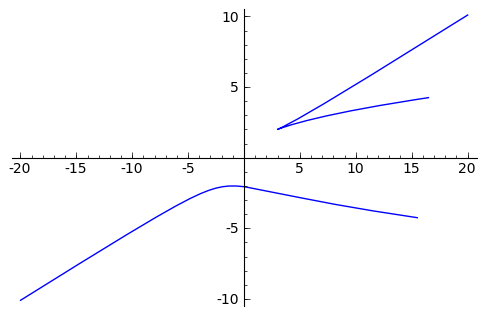
\includegraphics[width=9cm]{pictures_bitmap/figdevoir3exo2.png}

  \caption{La courbe de l'exercice \ref{exodevoir3-0002}}\label{figdevoir3exo2}
  \end{center}
 \end{figure}
\end{corrige}
